\chapter{Wartungsstrategien}\label{ch:pdm_theorie}
Die zunehmende Komplexität und Vernetzung moderner Systeme erfordert effizientere Wartungsstrategien. Predictive Maintenance nutzt die
enormen Datenmengen solcher Systeme, um drohende Defekte frühzeitig zu erkennen und Ausfälle zu verhindern. Dadurch können
Ausfallzeiten minimiert und die Lebensdauer der Systeme verlängert werden.

Im Vergleich zu traditionellen Ansätzen bietet Predictive Maintenance signifikante Vorteile,
doch auch die klassischen Methoden haben ihre Berechtigungen. Diese werden im Folgenden diskutiert.

\section{Traditionelle Wartungsansätze}\label{sec:trad_maintenance}
Zu den traditionellen Wartungsansätzen gehören die reaktive und die präventive Wartung. Bei der reaktiven oder auch korrektiven
Wartung wird, gemäß der Namensgebung, erst bei vollständigem Ausfall von Komponenten gehandelt.
Der Vorteil dieser Methode liegt in der sehr geringen Planung und Überwachung. Für Komponenten,
die nicht kritisch oder essenziell sind, oder die ein sehr geringes Ausfallrisiko aufweisen, kann die reaktive Wartung sinnvoll sein.
Für alle anderen Bestandteile bzw.~die Gesamtheit eines Systems ist sie jedoch höchst ineffizient, da Wartungsmaßnahmen erst dann
veranlasst und geplant werden, wenn das System ausfällt. Zudem gestaltet sich die Diagnose dann auch als potenziell schwierig, da die
Fehlerquelle noch gefunden werden muss~\cite{Abdelli2022}.

Demgegenüber steht die präventive Wartung, die Maßnahmen am Ende eines vorher festgelegten Zeitintervalls oder nach Ablauf einer
bestimmten Betriebsdauer festlegt. Diese Zeitintervalle werden beispielsweise anhand der Badewannenkurve~\cite[S.~4]{Andrews2002},
wie in \hyperref[fig:bathtub]{Abb.~\Ref*{fig:bathtub}} dargestellt, auf Basis von Erfahrungswerten oder empirischen Untersuchungen geschätzt.
Die Badewannenkurve ist eine Darstellung der Ausfallverteilung, die die Wahrscheinlichkeitsverteilung von mechanischen oder elektrischen
Defekten beschreibt. Dieser Ansatz hat gewisse Vorteile für Komponenten, die nicht im dauerhaften Betrieb sind, sofern ausreichend geschultes Personal vorhanden
ist mit genügend Zeit, die Wartungsarbeiten durchzuführen. Nachteile liegen im potenziell schlechten Timing der Wartungsarbeiten, die
entweder zu früh oder zu spät stattfinden. Ohne Überwachung des Systemzustands ist schwer absehbar, in welchem Stadium seiner Lebensdauer
sich ein System befindet, und Komponenten, die noch eine gewisse Zeit weiterlaufen könnten, werden zu früh ausgetauscht. Durch die Wartung
verkürzt sich auch die Betriebsdauer des ganzen Systems und verursacht vermeidbare Kosten~\cite{Scheffer2004}.

\begin{figure}[H]
    \centering
    \begin{tikzpicture}
        \node[anchor=south west,inner sep=0] (image) at (0,0) {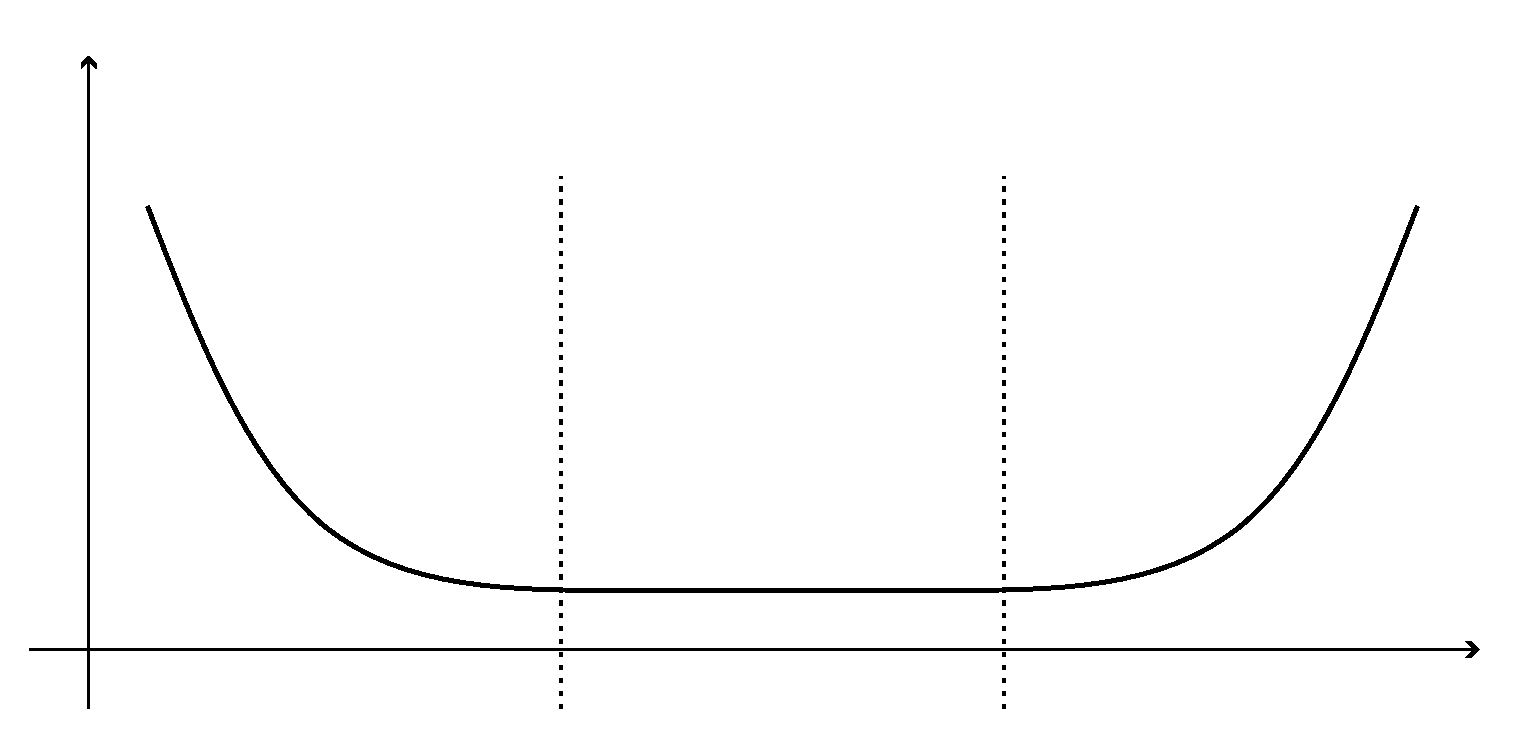
\includegraphics[width=\linewidth]{ch3_pdm_theorie/abbildungen/bathtub.pdf}};
        % Koordinatensystem für die Grafik
        \begin{scope}[x={(image.south east)},y={(image.north west)}]
            % Textpositionen anpassen:
            \node at (0.25,0.92) {\large\parbox{6cm}{Ausfallwahrscheinlichkeit}};
            \node at (0.88,0.05) {\large\centering Betriebsdauer};
            \node at (0.25,0.6) {\large\parbox{4cm}{\centering I\\Frühausfälle}};
            \node at (0.51,0.6) {\large\parbox{6cm}{\centering II\\normale Lebensdauer}};
            \node at (0.77,0.6) {\large\parbox{4cm}{\centering III\\Alterserscheinungen}};
        \end{scope}
    \end{tikzpicture}
    \caption{Badewannenkurve zur Visualisierung der Ausfallverteilung}
~\label{fig:bathtub}
\end{figure}

\section{Predictive Maintenance}
Nach Mobley~\Cite[S.~4]{Mobley2002} wird Predictive Maintenance als eine zustandsbasierte Wartungsstrategie definiert, die den
tatsächlichen Betriebszustand von Anlagen und Systemen überwacht, um Wartungsaktivitäten bedarfsgerecht zu planen.
Eine passende Analogie findet sich in der Medizin: Wenn der menschliche Körper Anzeichen einer bevorstehenden Krankheit zeigt, können
diese Symptome vom Arzt genutzt werden, um eine Diagnose zu stellen. Dementsprechend werden dann Maßnahmen ergeriffen, zum Beispiel
wird eine Behandlung eingeleitet oder Medikamente verordnet. Diese Zustandsüberwachung erlaubt es, dass Wartungsarbeiten zu einem
Zeitpunkt stattfinden können, der für alle Beteiligten passend ist und minimale Einschnitte in Produktions- oder Prozesslaufzeiten
bedeutet~\cite[S.~3]{Scheffer2004}.

Anhand von \hyperref[fig:pdm_workflow]{Abb.~\Ref*{fig:pdm_workflow}} ist zu erkennen, welche vereinfachten Schritte zur erfolgreichen
Implementierung eines Predictive Maintenance Systems erforderlich sind. Essentiell ist an erster Stelle eine adäquate Infrastruktur, die
sämtliche Zustandsparameter erfasst und gleichzeitig in der Lage ist, die erfassten Daten auch bereitzustellen. Es müssen im nächsten
Schritt Daten gesammelt werden, damit die im normalen Betriebszustand gültigen Schwellwerte ermittelt und festgelegt werden können.
Anhand dieser wird dann im laufenden, mittlerweile aufgenommenen Betrieb festgestellt, ob Abweichungen von den Parametern im Normalbetrieb
vorliegen. Demnach werden notwendige Wartungsarbeiten geplant und vorbereitet, wonach der Betrieb wieder ordnungsgemäß aufgenommen werden
kann.

\begin{figure}[H]
    \centering
    \begin{tikzpicture}
        \node[anchor=south west,inner sep=0] (image) at (0,0) {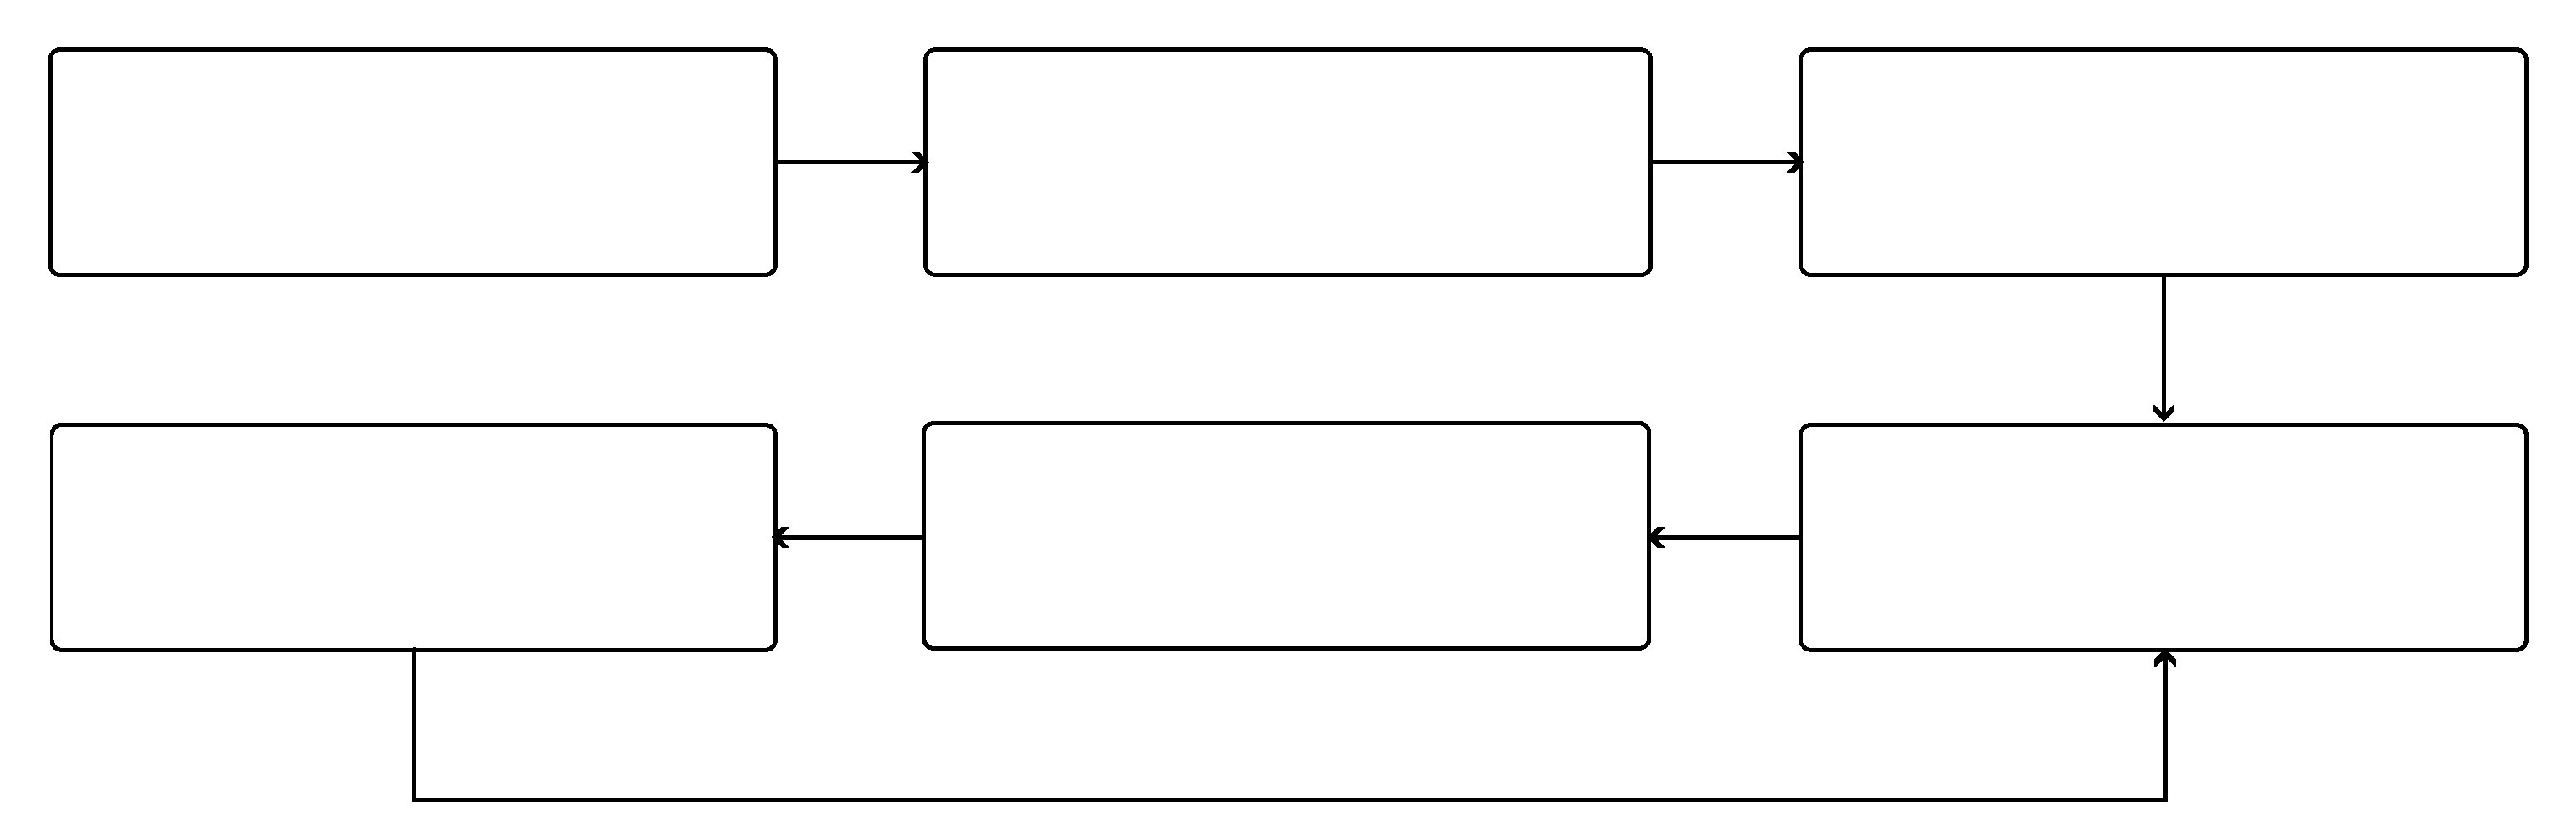
\includegraphics[width=\linewidth]{ch3_pdm_theorie/abbildungen/pdm_workflow.pdf}};
        % Koordinatensystem für die Grafik
        \begin{scope}[x={(image.south east)},y={(image.north west)}]
            % Textpositionen anpassen:
            \node at (0.16,0.815) {\large\parbox{6cm}{\centering Zustandsüberwachung\\einrichten}};
            \node at (0.5,0.815) {\large\parbox{6cm}{\centering Daten aggregieren}};
            \node at (0.84,0.815) {\large\parbox{6cm}{\centering Schwellwerte festlegen \&\\Parameter setzen}};
            \node at (0.84,0.35) {\large\parbox{6cm}{\centering normale\\Betriebsaufnahme}};
            \node at (0.5,0.35) {\large\parbox{6cm}{\centering Anomalien im\\Betrieb feststellen}};
            \node at (0.16,0.35) {\large\parbox{6cm}{\centering Wartungsarbeiten\\durchführen}};
        \end{scope}
    \end{tikzpicture}
    \caption{Workflow eines Predictive Maintenance Systems}
~\label{fig:pdm_workflow}
\end{figure}

Es stellt sich die Frage, welcher Anwendungsfall hauptsächlich interessant ist. In~\hyperref[ch:zielsetzung]{Kap.~\Ref*{ch:zielsetzung}}
wird bereits erläutert, in welchem Umfang eine Diagnose bzw.~Prognose gestellt werden soll. Vorrangig ist die Detektion von anomalem
Verhalten im laufenden Betrieb wie z.~B.~auftretende Alterserscheinungen oder Komponentenausfälle. Anhand dieser Anomalien soll durch
zusätzlichen menschlichen Input entschieden werden, ob und wann ein Wartungseinsatz notwendig ist.

Predictive Maintenance ist keineswegs eine neue Erscheinung. Der Ansatz und erste Methoden zur Umsetzung bestehen bereits seit den 70er
und 80er Jahren~\cite{Sandtorv1973, Renwick1985} mit Techniken wie beispielsweise der Vibrationsanalyse zur Zustandsbestimmung. Dabei
entwickelte sich der Fokus von Predictive Maintenance von lediglich der anfänglichen Überwachung durch die immer größer werdenden
Datenmengen hin zur ganzheitlichen Zustandsüberwachung. Durch technologische und industrielle Fortschritte wie Industrie 4.0 und dem
Internet of Things wurde die Umsetzung und Implementierung von Predictive Maintenance immer einfacher und kostengünstiger. Auf diese sog.
\textit{Enabling Technologies} wird in~\hyperref[sec:technologische_grundlagen]{Abs.~\Ref*{sec:technologische_grundlagen}} genauer
eingegangen.

Insgesamt zeigt sich das Konzept der Predictive Maintenance als natürliche Weiterentwicklung der traditionellen Wartungsansätze aufgrund
der einhergehenden technologischen Fortschritte. Während diese Arbeit lediglich Teilschritte zur Entwicklung eines Predictive Maintenance
Systems beitragen will, soll anhand der Erkenntnisse und Ergebnisse die Einführung und Nutzung eines solchen Systems die offensichtliche
Konsequenz sein.